\documentclass[10pt, a4paper]{article}

\usepackage{amssymb, amsmath}
\usepackage[utf8]{inputenc}
\usepackage[ngerman]{babel}
\usepackage{fancyhdr}
\usepackage{tikz}
\usepackage{fullpage}
\usepackage{graphicx}
\usepackage{alltt}

\usepackage{listings} 
\lstset{	numbers=left, 
		numberstyle=\tiny, 
		numbersep=5pt,
		stepnumber=2,
		showspaces=false,
		showstringspaces=false,
		tabsize=4,
		captionpos=b,
		backgroundcolor=\color{white},
		frame=single,
		language=PHP}

\pagestyle{fancy}
\setlength{\headheight}{12.4pt}
\setlength{\headsep}{1.5\headheight}

% 1. Person eintragen
\newcommand{\FirstAuthor}{Hasenauer}
\newcommand{\FirstAuthorFirstName}{Hannes}
\newcommand{\FirstAuthorMatnum}{0930213}

% 2. Person eintragen
\newcommand{\SecAuthor}{Fritzsch}
\newcommand{\SecAuthorFirstName}{Daniel}
\newcommand{\SecAuthorMatnum}{0930754}

% 3. Person eintragen
\newcommand{\ThirdAuthor}{Temmel}
\newcommand{\ThirdAuthorFirstName}{Hans Christian}
\newcommand{\ThirdAuthorMatnum}{0930308}

\newcommand{\AuthorFront}{{\normalsize
\begin{tabular}{|c|c|c|} \hline
\textbf{Nachname} & \textbf{Vorname}       & \textbf{Matrikelnummer} \\ \hline \hline
\FirstAuthor      & \FirstAuthorFirstName  & \FirstAuthorMatnum      \\ \hline
\SecAuthor        & \SecAuthorFirstName    & \SecAuthorMatnum        \\ \hline
\ThirdAuthor      & \ThirdAuthorFirstName  & \ThirdAuthorMatnum      \\ \hline
\end{tabular}}}

\author{\AuthorFront}
\newcommand{\Author}{\FirstAuthorMatnum, \SecAuthorMatnum,
                     \ThirdAuthorMatnum}

\date{} % Kein Datum angegeben
\fancyfoot{} % Seitenzahl unten nicht anzeigen

\lhead{Modern Information Systems}
\chead{\Author}
\rhead{Seite \thepage}

\title{Modern Information Systems WS 11/12}

\begin{document}

%%%%%%%%%%%%%%%%%%%%%%%%%%%%%%%%%%%%%%%%%%%%%%%%%%%%%%%%%%%%%%%%%%%%%%%%%%%%%%%%

\newcounter{ale}
\newcommand{\abc}{\item[\alph{ale})]\stepcounter{ale}}
\newenvironment{liste}{\begin{itemize}}{\end{itemize}}
\newcommand{\aliste}{\begin{liste} \setcounter{ale}{1}}
\newcommand{\zliste}{\end{liste}}
\newenvironment{abcliste}{\aliste}{\zliste}

%%%%%%%%%%%%%%%%%%%%%%%%%%%%%%%%%%%%%%%%%%%%%%%%%%%%%%%%%%%%%%%%%%%%%%%%%%%%%%%%

\maketitle
\thispagestyle{fancy}

%%%%%%%%%%%%%%%%%%%%%%%%%%%%%%%%%%%%%%%%%%%%%%%%%%%%%%%%%%%%%%%%%%%%%%%%%%%%%%%%

\tableofcontents
\pagebreak

\section{Database Schema}

\subsection{Entity-Relationship Diagram}

\begin{figure}[htb]
	\centering
	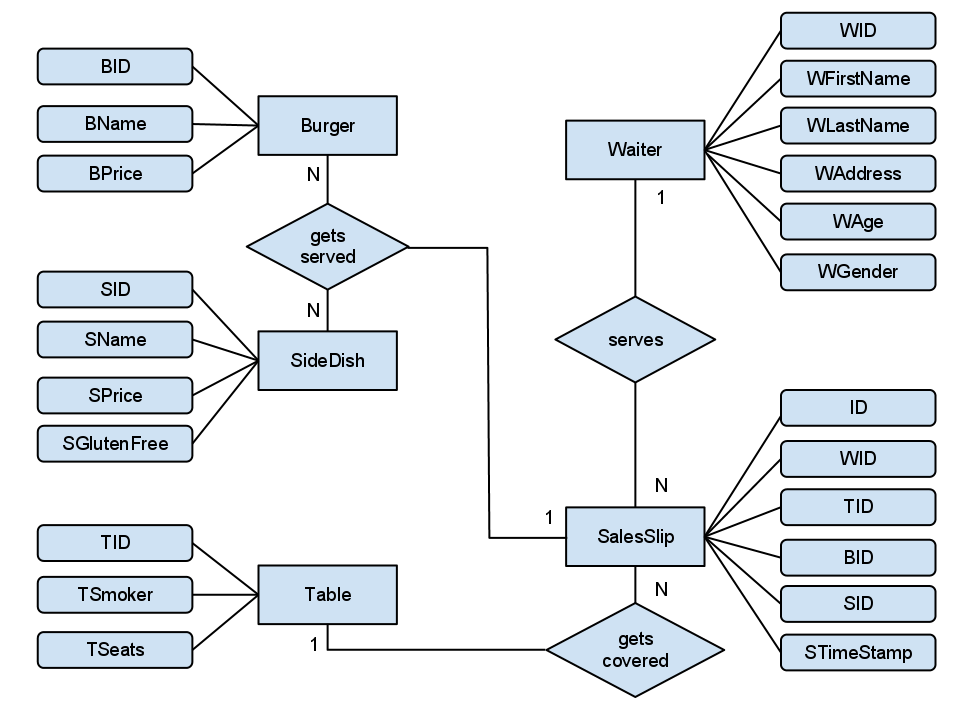
\includegraphics[scale=0.49]{fig/entity_relationship_diagram.png}
	\caption{Entity-Relationship Diagram}
\end{figure}

\subsection{Domains}

\begin{tabular}[ht]{| p{4.9cm} | p{4.9cm} | p{4.9cm} |}
\hline
  	Name 		& DataType 	& Description\\
\hline\hline
  	WID                	& Integer 		& Waiter ID\\
  	WFirstName 	& String   		& Firstname of the waiter\\
  	WLastName 	& String    		& Lastname of the waiter\\
 	WAddress    	& String    		& Address of the waiter\\
 	WAge           	& Integer   	& Age of the waiter\\
 	WGender     	& Integer   	& Gender of the waiter\\
\hline
  	TID                	& Integer   	& Table ID\\
  	TSmoker      	& Boolean	& Smokertable?\\
  	TSeats      		& Integer 		& Amount of seats\\
\hline
  	BID                	& Integer   	& Burger ID\\
  	BName      	& String		& Name of the burger\\
  	BPrice      		& Integer 		& Price of the burger\\
\hline
  	SID                	& Integer   	& Sidedish ID\\
  	SName      	& String		& Name of the sidedish\\
  	SPrice      		& Integer 		& Price of the sidedish\\
	SGlutenfree      	& Boolean 	& Glutenfree?\\
\hline
  	ID                	& Integer   	& Sales Slip ID\\
  	WID                	& Integer 		& Waiter ID\\
  	TID                	& Integer   	& Table ID\\
  	BID                	& Integer   	& Burger ID\\
  	SID                	& Integer   	& Sidedish ID\\
	STimeStamp    	& TimeStamp   	& The actual timestamp\\
\hline
\end{tabular}

\subsection{Relations}

\begin{tabular}[ht]{| p{2.8cm} | p{2.8cm} | p{2.8cm} | p{2.8cm} | p{2.8cm} |}
\hline
  	Waiter 			& Table 			& Burger			& SideDish 		& SalesSlip\\
\hline\hline
	\underline{WID}	& \underline{TID}     	& \underline{BID}	& \underline{SID}	& \underline{ID}\\
	WFirstName		& TSmoker     		& BName			& SName			& WID\\
	WLastName		& TSeats     		& BPrice			& SPrice			& TID\\
	WAddress			& 		     		&				& SGlutenFree		& BID\\
	WAge			& 		     		&				& 				& SID\\
	WGender			& 		     		&				& 				& STimeStamp\\
\hline
\end{tabular}

\subsubsection{Additional Description}

The domains WID, TID, BID and SID are the foreign keys in the relation SalesSlip.

\subsection{Functional Dependencies}

\begin{itemize}
	\item Waiter(\underline{WID}, WFirstName, WLastName, WAddress, WAge, WGender)
		\subitem - WID $\rightarrow$ WFirstName
		\subitem - WID $\rightarrow$ WLastName
		\subitem - WID $\rightarrow$ WAddress
		\subitem - WID $\rightarrow$ WAge
		\subitem - WID $\rightarrow$ WGender
	\item Table(\underline{TID}, TSmoker, TSeats)
		\subitem - TID $\rightarrow$ TSmoker
		\subitem - TID $\rightarrow$ TSeats
		
	\pagebreak	
	
	\item Burger(\underline{BID}, BName, BPrice)
		\subitem - 	BID $\rightarrow$ BName
		\subitem - 	BID $\rightarrow$ BPrice
	\item SideDish(\underline{SID}, SName, SPrice, SGlutenFree)
		\subitem - SID $\rightarrow$ SName
		\subitem - SID $\rightarrow$ SPrice
		\subitem - SID $\rightarrow$ SGlutenFree
	\item SalesSlip(\underline{ID}, WID, TID, BID, SID, STimeStamp)
		\subitem - ID $\rightarrow$ WID
		\subitem - ID $\rightarrow$ TID
		\subitem - ID $\rightarrow$ BID
		\subitem - ID $\rightarrow$ SID
		\subitem - ID $\rightarrow$ STimeStamp	
\end{itemize}

\subsubsection{Additional Description}

Every domain in the relation is only identifiable by a unique primary key. Therefore there are no indirect key dependencies and the database is in the 3rd normal form.

\pagebreak
\section{Practical Implementation}

For all primary keys auto increment values are used. This is done to assign a unique identifier to every relation who contains a primary key automatically.

\subsection{Waiter}

\subsubsection{Relation}

\begin{verbatim}
CREATE TABLE IF NOT EXISTS `Waiter` (
	`WID`		int(5) unsigned NOT NULL AUTO_INCREMENT,
  	`WFirstName` 	varchar(30) NOT NULL,
  	`WLastName`  	varchar(30) NOT NULL,
  	`WAddress`   	varchar(100) NOT NULL,
  	`WAge`       	int(3) NOT NULL,
  	`WGender`    	varchar(10) NOT NULL,
  	PRIMARY KEY (`WID`)
);
\end{verbatim}

\subsubsection{Data}

\begin{verbatim}
INSERT INTO `Waiter` (`WFirstName`, `WLastName`, `WAddress`, `WAge`, `WGender`) VALUES
  	('Daniel', 'Fritzsch', 'Daniels Address', 20, 'male');
INSERT INTO `Waiter` (`WFirstName`, `WLastName`, `WAddress`, `WAge`, `WGender`) VALUES
  	('Hannes', 'Hasenauer', 'Hannes Address', 23, 'male');
INSERT INTO `Waiter` (`WFirstName`, `WLastName`, `WAddress`, `WAge`, `WGender`) VALUES
  	('Hans Christian', 'Temmel', 'Hans Christians Address', 25, 'male');
INSERT INTO `Waiter` (`WFirstName`, `WLastName`, `WAddress`, `WAge`, `WGender`) VALUES
  	('Sandra', 'Steal', 'Sandras Address', 15, 'female');
\end{verbatim}

\subsubsection{Screenshot}

\begin{figure}[htb]
	\centering
	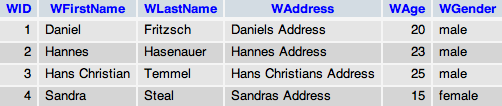
\includegraphics[scale=0.9]{fig/waiter.png}
	\caption{Waiter}
\end{figure}

\subsection{Table}

\subsubsection{Relation}

\begin{verbatim}
CREATE TABLE IF NOT EXISTS `Table` (
  	`TID`      		int(5) unsigned NOT NULL AUTO_INCREMENT,
  	`TSmoker`  	tinyint(1) NOT NULL DEFAULT FALSE,
  	`TSeats`   		int(2) unsigned NOT NULL,
  	PRIMARY KEY (`TID`)
);
\end{verbatim}

\subsubsection{Data}

\begin{verbatim}
-- NonSmoking Tables
INSERT INTO `Table` (`TSeats`) VALUES (4);
INSERT INTO `Table` (`TSeats`) VALUES (4);
INSERT INTO `Table` (`TSeats`) VALUES (2);
INSERT INTO `Table` (`TSeats`) VALUES (5);

-- Smoking Tables
INSERT INTO `Table` (`TSmoker`, `TSeats`) VALUES (true, 4);
INSERT INTO `Table` (`TSmoker`, `TSeats`) VALUES (true, 2);
INSERT INTO `Table` (`TSmoker`, `TSeats`) VALUES (true, 5);
\end{verbatim}

\subsubsection{Screenshot}

\begin{figure}[htb]
	\centering
	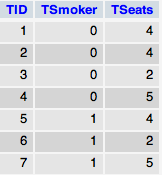
\includegraphics[scale=0.9]{fig/table.png}
	\caption{Table}
\end{figure}

\subsection{Burger}

\subsubsection{Relation}

\begin{verbatim}
CREATE TABLE IF NOT EXISTS `Burger` (
  	`BID`    	int(5) unsigned NOT NULL AUTO_INCREMENT,
  	`BName`  	varchar(25) NOT NULL,
  	`BPrice` 	float(4,2) NOT NULL,
  	PRIMARY KEY (`BID`)
);
\end{verbatim}

\subsubsection{Data}

\begin{verbatim}
INSERT INTO `Burger` (`BName`, `BPrice`) VALUES
  	('Manhattan Burger', 6);
INSERT INTO `Burger` (`BName`, `BPrice`) VALUES
  	('NewYork Classic', 6.5);
INSERT INTO `Burger` (`BName`, `BPrice`) VALUES
  	('Extra Meat Burger', 8);
INSERT INTO `Burger` (`BName`, `BPrice`) VALUES
  	('Hot Chicken Burger', 7.25);
INSERT INTO `Burger` (`BName`, `BPrice`) VALUES
  	('Austrian Burger', 7.5);
\end{verbatim}

\subsubsection{Screenshot}

\begin{figure}[htb]
	\centering
	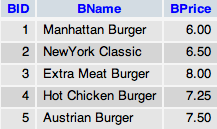
\includegraphics[scale=0.9]{fig/burger.png}
	\caption{Burger}
\end{figure}

\subsection{SideDish}

\subsubsection{Relation}

\begin{verbatim}
CREATE TABLE IF NOT EXISTS `SideDish` (
  	`SID`         		int(5) unsigned NOT NULL AUTO_INCREMENT,
  	`SName`       	varchar(15) NOT NULL,
  	`SPrice`      	float(4,2) NOT NULL,
  	`SGlutenFree` 	tinyint(1) NOT NULL DEFAULT FALSE,
  	PRIMARY KEY (`SID`)
);
\end{verbatim}

\subsubsection{Data}

\begin{verbatim}
INSERT INTO `SideDish` (`SName`, `SPrice`, `SGlutenFree`) VALUES
  	('Pommes', 2.5, true);
INSERT INTO `SideDish` (`SName`, `SPrice`) VALUES
  	('Potatoes', 2);
INSERT INTO `SideDish` (`SName`, `SPrice`) VALUES
  	('Potato Stripes', 2.7);
INSERT INTO `SideDish` (`SName`, `SPrice`, `SGlutenFree`) VALUES
  	('Rice', 2, true);
\end{verbatim}

\subsubsection{Screenshot}

\begin{figure}[htb]
	\centering
	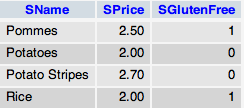
\includegraphics[scale=0.9]{fig/sidedish.png}
	\caption{SideDish}
\end{figure}

\subsection{SalesSlip}

\subsubsection{Relation}

\begin{verbatim}
CREATE TABLE IF NOT EXISTS `SalesSlip` (
  	`ID`       		int(100) unsigned NOT NULL AUTO_INCREMENT,
  	`WID`        		int(5) unsigned NOT NULL,
  	`TID`        		int(5) unsigned NOT NULL,
  	`BID`        		int(5) unsigned,
  	`SID`        		int(5) unsigned,
  	`STimeStamp` timestamp NOT NULL DEFAULT CURRENT_TIMESTAMP,
  	PRIMARY KEY (`ID`)
);
\end{verbatim}

\subsubsection{Data}

\begin{verbatim}
INSERT INTO `SalesSlip` (`WID`, `TID`, `BID`, `SID`) VALUES
  	(1, 5, 1, 1);
INSERT INTO `SalesSlip` (`WID`, `TID`, `BID`, `SID`) VALUES
  	(1, 6, 2, 2);
INSERT INTO `SalesSlip` (`WID`, `TID`, `BID`, `SID`) VALUES
  	(1, 7, 3, 3);
INSERT INTO `SalesSlip` (`WID`, `TID`, `BID`, `SID`, `STimeStamp`) VALUES
  	(1, 5, 0, 2, '2010-11-18 12:00:30');
INSERT INTO `SalesSlip` (`WID`, `TID`, `BID`, `SID`) VALUES
  	(1, 6, 1, 3);
INSERT INTO `SalesSlip` (`WID`, `TID`, `BID`, `SID`) VALUES
  	(1, 7, 3, 1);
INSERT INTO `SalesSlip` (`WID`, `TID`, `BID`, `SID`, `STimeStamp`) VALUES
  	(2, 3, 5, 2, '2009-08-10 10:04:30');
INSERT INTO `SalesSlip` (`WID`, `TID`, `BID`, `SID`) VALUES
  	(2, 4, 3, 1);
INSERT INTO `SalesSlip` (`WID`, `TID`, `BID`, `SID`, `STimeStamp`) VALUES
  	(2, 4, 1, 3, '2011-04-03 16:00:42');
INSERT INTO `SalesSlip` (`WID`, `TID`, `BID`, `SID`) VALUES
  	(2, 6, 2, 2);
INSERT INTO `SalesSlip` (`WID`, `TID`, `BID`, `SID`, `STimeStamp`) VALUES
  	(3, 2, 2, 2, '2008-06-05 14:05:42');
INSERT INTO `SalesSlip` (`WID`, `TID`, `BID`, `SID`) VALUES
  	(3, 2, 1, 4);
INSERT INTO `SalesSlip` (`WID`, `TID`, `BID`, `SID`) VALUES
  	(4, 1, 4, 3);
INSERT INTO `SalesSlip` (`WID`, `TID`, `BID`, `SID`) VALUES
  	(4, 1, 2, 4);
INSERT INTO `SalesSlip` (`WID`, `TID`, `BID`, `SID`, `STimeStamp`) VALUES
  	(4, 1, 5, 2, '2010-09-14 17:00:51');
\end{verbatim}

\pagebreak
\subsubsection{Screenshot}

\begin{figure}[htb]
	\centering
	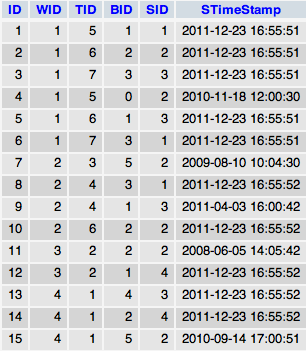
\includegraphics[scale=0.9]{fig/salesslip.png}
	\caption{SalesSlip}
\end{figure}

\section{XSL}
The user is able to get a overall statistic of all waiters and their serves. There are 2 stylesheets available. One stylesheet for an overview over all tables and one stylesheet for an overview over just the table where smoking is allowed. There are also 2 methods for transformation, either the result is created on the server or on the client side.

\pagebreak
\section{Relevant Code Snippets}
\subsection{Adding a new Burger}

\begin{lstlisting}[caption=addBurger.php]
<form action="addBurger.php" method="POST">
    <table width="600" border="0" cellspacing="0" cellpadding="0">
      <tr>
        <td width="128">Name:</td>
        <td width="472"><input type="text" name="bName"></input></td>
      </tr>
      <tr>
        <td>Price</td>
        <td><input type="text" name="bPrice"></input></td>
      </tr>
    </table>
    
    <input type="submit" value="Submit"></input>
</form>

<?php
    if (isset ($_POST["bName"]) && $_POST["bPrice"]) {
        
        $bName  = $_POST["bName"];
        $bPrice = $_POST["bPrice"];
        $query  = "INSERT INTO `Burger` (`BID`, `BName`, `BPrice`)
                   VALUES (NULL, '$bName', '$bPrice');";
        
        mysql_query($query) or die (mysql_error());
        echo ("Burger $bName has been added to database");
    }
?>
\end{lstlisting}
This file is used to add a new burger to the database. It is necessary to use a valid value [0-99] as price.

\subsection{Delete a Burger}

\begin{lstlisting}[caption=deleteBurger.php]
<form action="deleteBurger.php" method="POST">
<?php
    if(isset ($_POST["burger"])) {
        $burger = $_POST["burger"];
        $query  = "DELETE FROM `Burger` WHERE BName='$burger';";
        
        mysql_query($query) or die (mysql_error());
    }
    $burgers = mysql_query("select * from `Burger`;") or die (mysql_error());
?>

<select name="burger">
<?php
    while($burger = mysql_fetch_array($burgers)) {
        echo ('<option value="' . $burger["BName"] . '">' . 
            $burger["BName"] . '</option>');
    }    
?>
</select>

<input type="submit" value="delete">
</form>

<?php
    if(isset ($_POST["burger"])) {
        $burger = $_POST["burger"];
        
        echo ("'$burger' has been deleted!");
    }
?>
\end{lstlisting}
This file is used to delete an existing burger from the database.

\subsection{Get burgers that are served by a given waiter to a specific table}

\begin{lstlisting}[caption=getBurgers.php]
<form action="getBurgers.php" method="POST">

<?php
    $waiters = mysql_query("select * from `Waiter`") or die(mysql_error());
    $tables  = mysql_query("SELECT * from `Table`")  or die(mysql_error());
?>

<select name="waiter">
    <?php
        while($waiter = mysql_fetch_array($waiters)) {
            if ($_POST["waiter"] == $waiter["WID"]) {
                echo '<option selected = yes value="'.$waiter["WID"].'">'.
                    $waiter["WLastName"]." ".$waiter["WFirstName"].
                    '</option>';
            } else {
                echo '<option value="'.$waiter["WID"].'">' .
                    $waiter["WLastName"]." ".$waiter["WFirstName"].
                    '</option>';
            }
        }
    ?>
    
</select>
<select name="table">
    <?php
        while($table = mysql_fetch_array($tables)) {
            if ($_POST["table"] == $table["TID"]) {
                echo '<option selected = yes value="'.$table["TID"].'">'.
                	"Table Number: ".$table["TID"].'</option>';
            } else {
                echo '<option value="'.$table["TID"].'">'."Table Number: ".
                	$table["TID"].'</option>'; 
            }
        }
    ?>


<?php
    
    if (isset ($_POST["waiter"]) && isset ($_POST["table"])) {
        
        $wid    = $_POST["waiter"];
        $tid    = $_POST["table"];
        $waiter = mysql_query("select * from Waiter where WID = $wid");
        $name   = mysql_fetch_object($waiter); 
        
        $result = mysql_query("select BName from Burger where BID in 
                                  (select BID from SalesSlip where 
                                  	WID = $wid and TID = $tid)");
        
        while ($burger = mysql_fetch_array($result)) {
            echo $burger["BName"] . " at table " . $tid . " by " 
                    . $name->WFirstName . " " . $name->WLastName;
        } 
    }
?>
\end{lstlisting}
Gets all burgers that are served by a given waiter to a specific table. 

\subsection{Get all burgers that have been served by a a specific waiter}

\begin{lstlisting}[caption=waiterStatistic.php]
<form action="waiterStatistic.php" method="POST">
  <table width="600" border="0" cellspacing="0" cellpadding="0">
  <tr>
    <td width="125">Waiter:</td>
    <td width="475"><?php        
    $waiters = mysql_query("select * from Waiter") or die (mysql_error());
?>
    
<select name="waiter">            
    <?php
        while ($waiter = mysql_fetch_array($waiters)) {
            if ($_POST["waiter"] == $waiter["WID"]) {
                echo '<option selected = yes value = "'.$waiter["WID"].'">'. 
                      $waiter["WLastName"]." ".$waiter["WFirstName"].
                      '</option>';
            } else {
                echo '<option value = "'.$waiter["WID"].'"> '. 
                      $waiter["WLastName"]." ".$waiter["WFirstName"].
                      '</option>';
            }
        }
    ?>
</select>
</td>
  </tr>
  <tr>
    <td>Smoker Table:</td>
    <td>
    
    
    <?php
   	if (isset ($_POST["smokertable"]))
        		echo '<input type="checkbox" name="smokertable" checked>';
    	else
        		echo '<input type="checkbox" name="smokertable">';
    ?>
    </td>
  </tr>
</table>

</form>
<?php
    if (isset ($_POST["waiter"])) {
        $wid = $_POST["waiter"];
        
        if (isset($_POST["smokertable"])) 
            $smoker = 1;
        else
            $smoker = 0;
            
        $result = 
        		mysql_query("SELECT * FROM Burger WHERE BID IN 
                   			(SELECT BID FROM `SalesSlip` WHERE WID = $wid 
							AND TID IN (SELECT TID FROM  `Table` WHERE 
							TSmoker = $smoker AND TID IN 
                           	(SELECT TID FROM `SalesSlip` WHERE WID = $wid))
							)");
                   
        while ($burger = mysql_fetch_array($result)) {
            echo $burger["BName"]; ?><br><?php
        }        
    }
?>
\end{lstlisting}
You can choose a waiter to see the statistic of the Burgers that have been served by him. Additionally you 
can check or uncheck to differ from smoker and non-smoker tables.

\subsection{Update the price of a burger}

\begin{lstlisting}[caption=updateBurgerPrice.php]
<form action="updateBurgerPrice.php" method="POST">
<table width="600" border="0" cellspacing="0" cellpadding="0">
  <tr>
    <td width="40">Burger:</td>
    <td width="475">
    <?php
        $burgers = mysql_query("select * from `Burger`;") 
        			or die (mysql_error());
    ?>
    <select name="burger" onchange="this.form.submit()">
    <?php 
        if (!isset($_POST["burger"])) {   
    ?>
    <option>-</option>
    
    
    <?php }
        while($burger = mysql_fetch_array($burgers)) {
            if ($_POST["burger"] == $burger["BID"]) {
                echo ('<option selected value="' . $burger["BID"] . '">' . 
                      $burger["BName"] . '</option>');
            } else {
                echo ('<option value="' . $burger["BID"] . '">' . 
                      $burger["BName"] . '</option>'); 
            }
        } 
    ?>

<?php }
    if (!isset($_POST["burger"]) && !isset($_POST["updatePrice"]))
        return;
    
    if (!isset($_POST["updatePrice"])){
        $bid = $_POST["burger"];
        $result = mysql_query("select * from `Burger` where BID = $bid");
        $price = mysql_fetch_array($result);
        echo $price["BName"] . " currently is " . $price["BPrice"] . "$";  
    }
?>

<form action="updateBurgerPrice.php" method="POST">
    If you want to change the price of the currently selected Burger enter 
    the new value here: <br>
    <?php   
        $bid = $_POST["burger"];
        echo '<input type="hidden" name="burger" value="'.$bid.'">';
    ?>
    <input type="text" name="updatePrice"></input> [0-99] <br>
    <br />
    <input type="submit" value="update">
</form>

<?php
    if (isset($_POST["updatePrice"])) {
        $newPrice = $_POST["updatePrice"];
        $bid = $_POST["burger"];
        $result = mysql_query("select * from `Burger` where BID = $bid");
        $name = mysql_fetch_array($result);
        
        if (is_numeric($newPrice) && $newPrice >=0 && $newPrice <= 99) {
            mysql_query("UPDATE `Burger` SET BPrice='$newPrice' 
            WHERE BID=$bid");
            
            echo"Changed the price of ".$name["BName"]." to ".$newPrice."$"; 
        } else
            echo "Please enter the price as an integer value [0-99]";
    }
?>
\end{lstlisting}
You can choose any Burger from a Dropdown menu and change its price. The new value also has to be valid [0-99].

\end{document}